\begin{frame}[fragile]{Architecture}
\begin{lstlisting}
fn update(bodies: &mut [RigidBody], dt: f64) {
    −\color{red}{integrate}−(bodies, dt);
    let collisions = −\color{red}{detect\_collisions}−(bodies, dt);
    let forces = −\color{red}{compute\_forces}−(bodies, collisions, dt);
    −\color{red}{apply\_forces}−(bodies, forces, dt);
}
\end{lstlisting}

\only<2> {
    \begin{figure}[h]
        \begin{center}
            \includegraphics[scale=0.5]{rust}
            \caption{Cet exemple est écrit en Rust \href{www.rust-lang.org}{www.rust-lang.org}}
        \end{center}
    \end{figure}
}

\end{frame}

\begin{frame}[fragile]{Architecture}
\vfill
\begin{center}
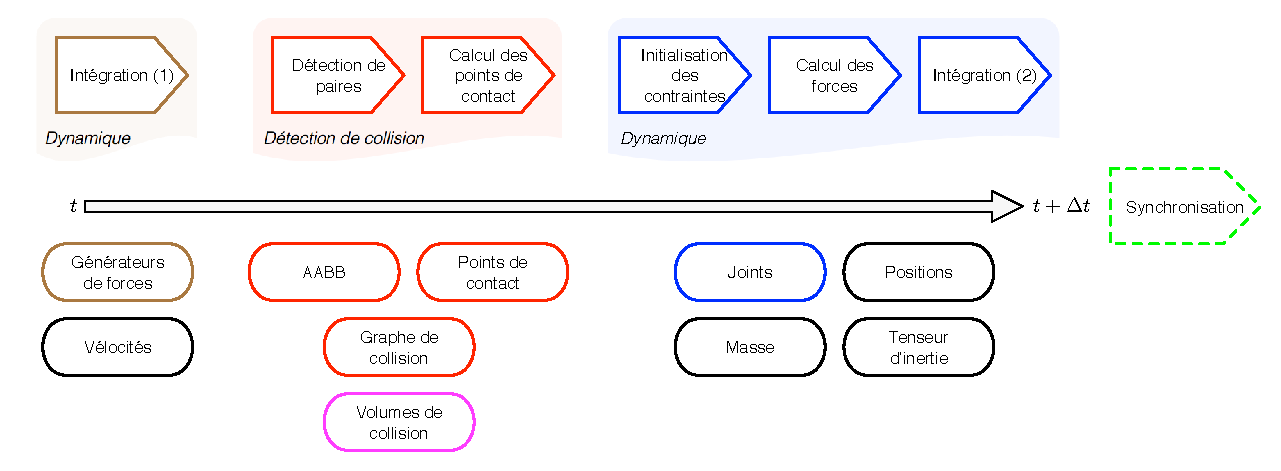
\includegraphics[scale=0.5]{workflow}
\end{center}
\vfill
\end{frame}
